\section{Сравнение полученных реализаций}
Проведем анализ производительности полученных версий анализатора. В качестве 
данных для тестирования возьмем выражения вида 
$\underbrace{2 + 2 + 2 + \cdots + 2}_{n}$ для $n = 1 \dots 100$ с шагом 1. Для 
вычисления времени выполнения воспользуемся библиотекой \texttt{time} 
Python 3.9.5. Автоматизацию обеспечим с помощью библиотеки \texttt{subprocess}. 
Получим следующий код:
\inputminted{python}{requirements/src/test.py}

Кроме того, отметим, что в ранее написанные программы были внесены некоторые 
изменения для проведения эксперимента. Ознакомиться с ними можно в приложении А.

Ознакомиться с полным исходным кодом программы, осуществляющей исследование 
производительности можно в приложении \ref{app:B}.

Для большей наглядности графики интерполированы полиномом с помощью функции 
\texttt{polyfit} библиотеки \texttt{numpy}.

Ознакомиться с полным исходным кодом программы, осуществляющей анализ полученных 
результатов можно в приложении \ref{app:C}.

Результаты исследования изображены на рис. \ref{img:benchmark}:
\begin{figure}[H]
    \centering
    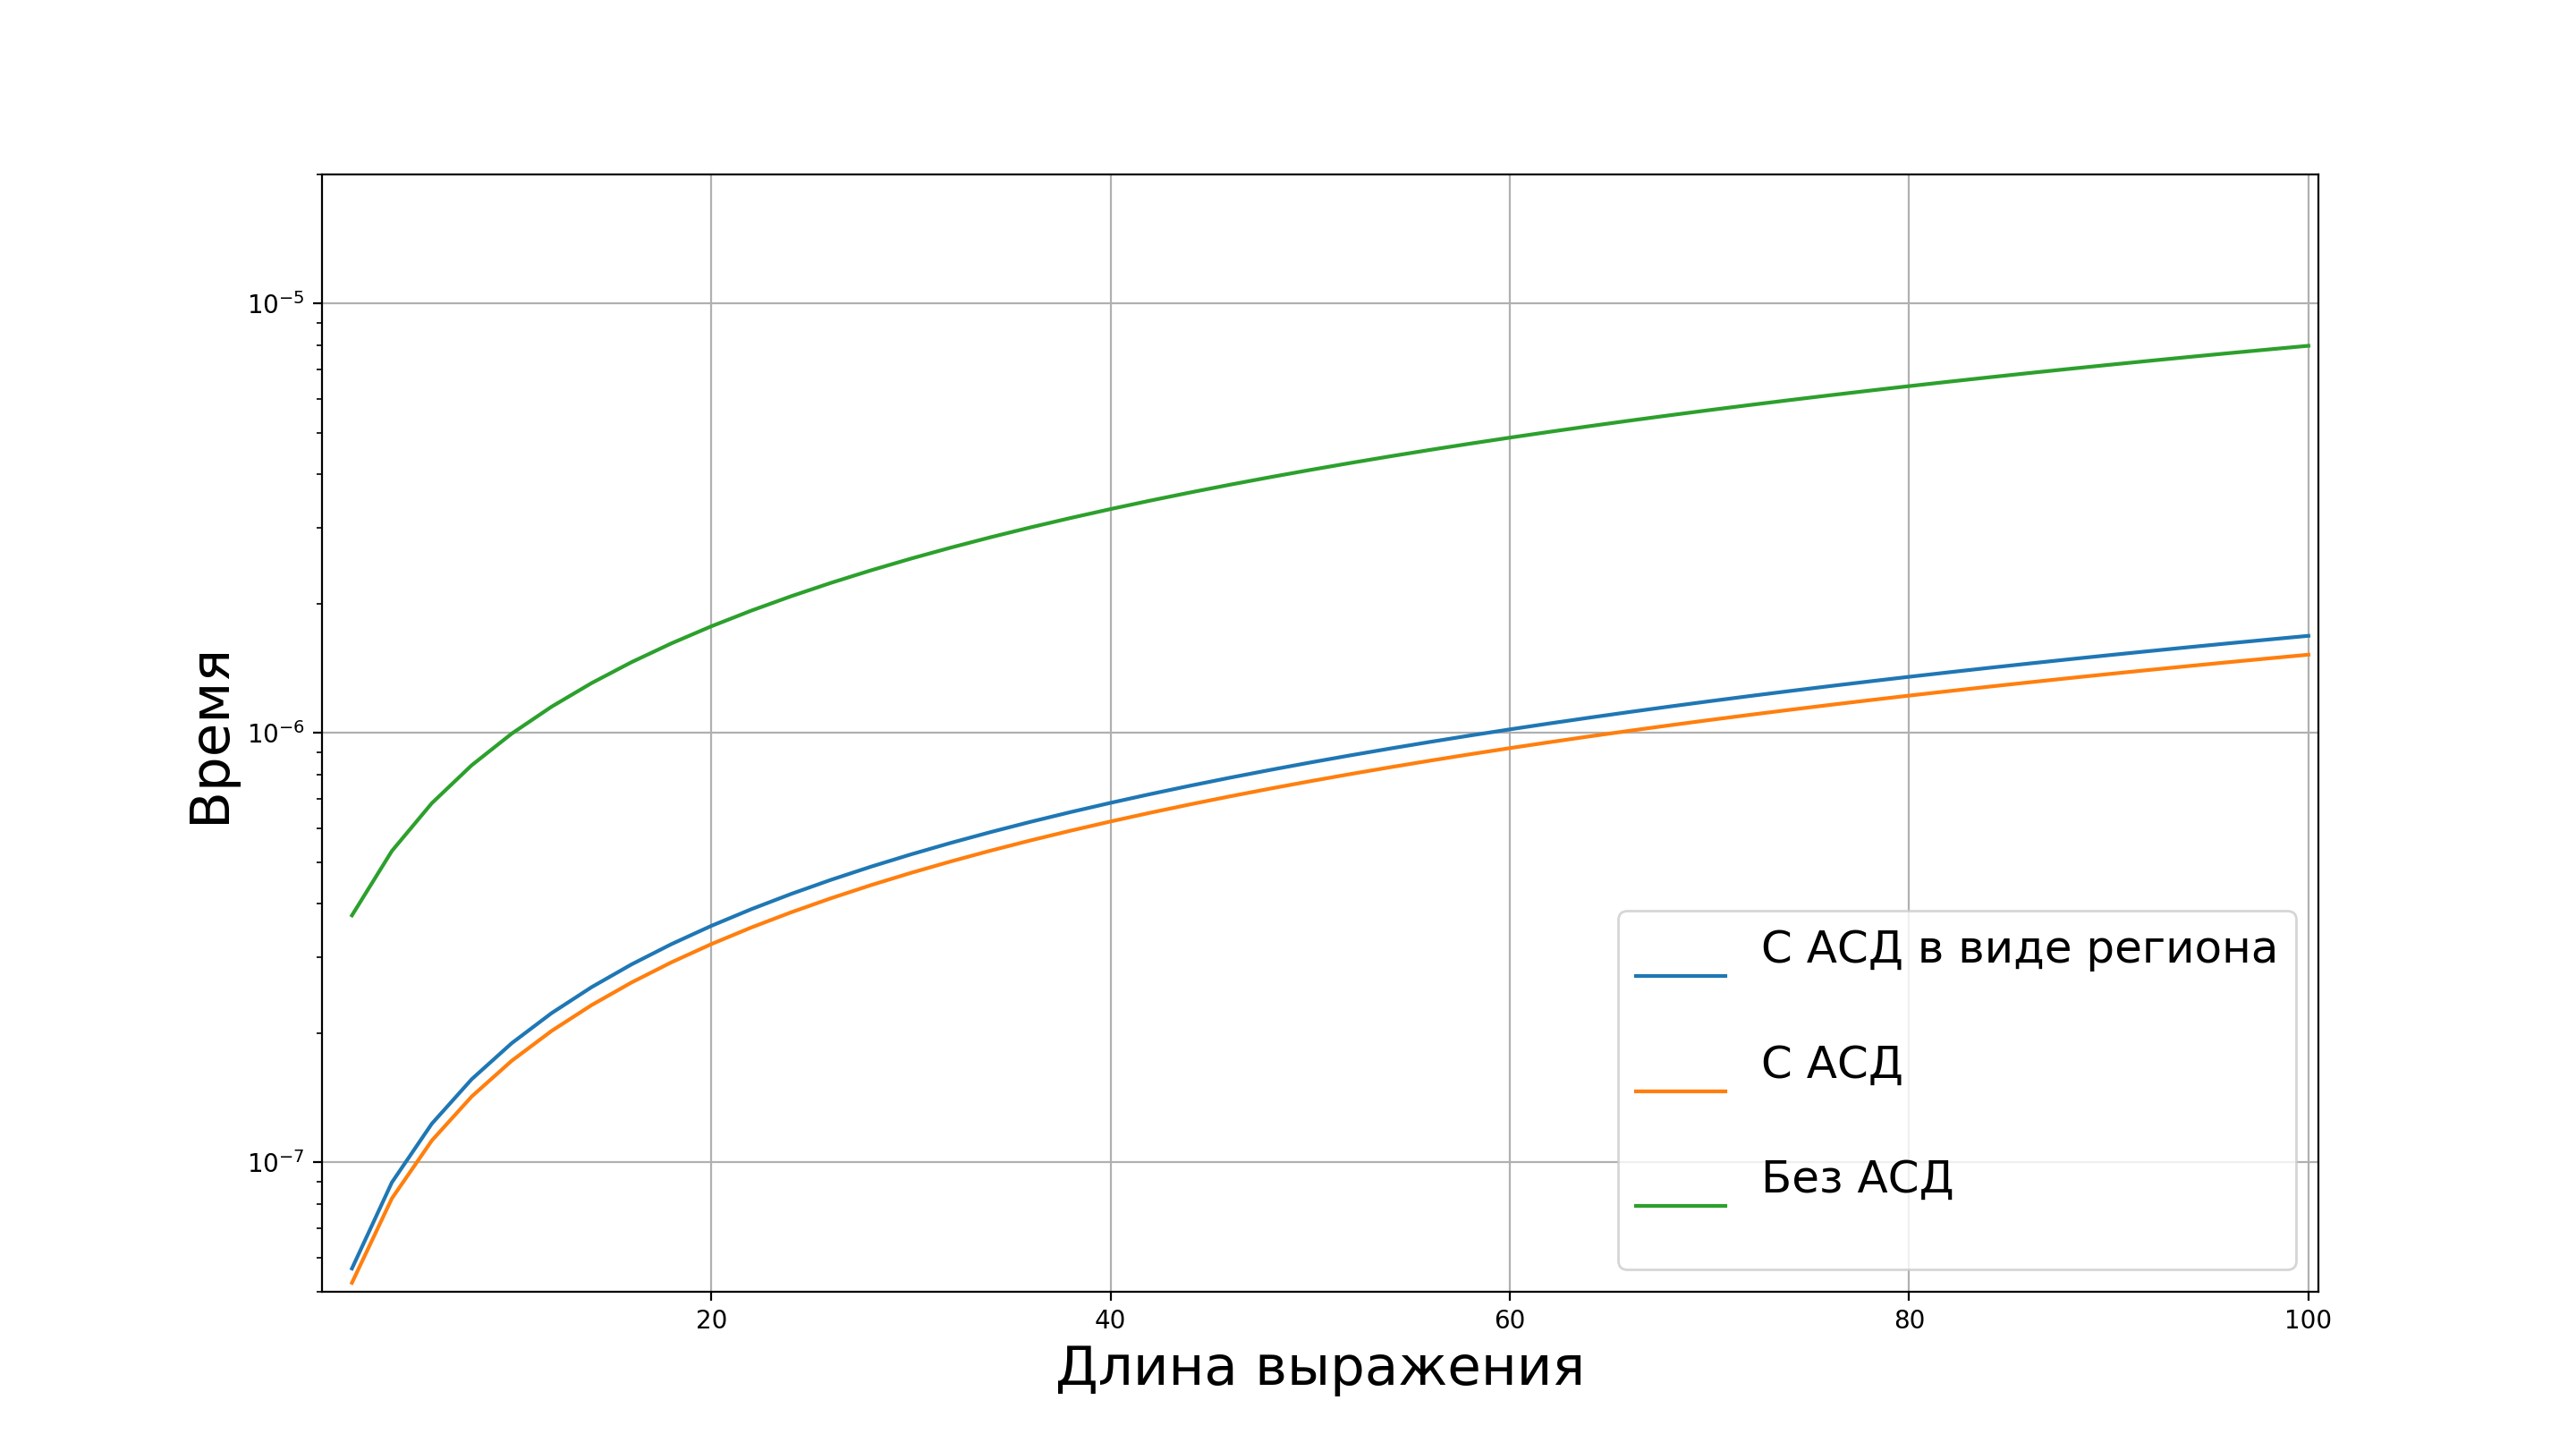
\includegraphics[width=\textwidth]{benchmark.png}
    \caption{Сравнение полученных результатов}
    \label{img:benchmark}
\end{figure} 
Исследование показало, что использование абстрактных синтаксических деревьев 
позволяет уменьшить время работы программы более чем в 5 раз, что существенно 
заметно для выражений любой длины.

Также из графиков видно, что в рамках данной работы не удалось добиться большей 
производительности при управлении памятью на основе регионов. Тем не менее, она 
все еще может считаться более предпочительной ввиду перечисленных ранее 
преимуществ.